\documentclass{article}
\usepackage[utf8]{inputenc}
\usepackage[german]{babel}
\usepackage{graphicx}
\usepackage[top=3cm, margin=1cm]{geometry}
\usepackage{listings}
\usepackage{hyperref}

\title{MTCG: Intermediate Protokoll}
\author{Rentenberger Lorenz}
\date{\today}

\begin{document}

\maketitle

\section{Projektübersicht}
Das Monster Trading Card Game (MTCG) ist eine REST-API Implementierung eines Kartenspiels. Die Anwendung ermöglicht Benutzern, sich zu registrieren, Karten zu sammeln, Decks zusammenzustellen und gegen andere Spieler anzutreten.

\subsection{GIT}
Link zum Github-Repository: \url{https://github.com/LRenTi/BIF3_SWEN1}

\section{Technische Entscheidungen}

\subsection{Architektur}
Die Anwendung folgt einer dreischichtigen Architektur:
\begin{itemize}
    \item API-Schicht (MTCG.Api): Behandelt HTTP-Requests und Routing
    \item Core-Schicht (MTCG.Core): Enthält die Geschäftslogik und Entitäten
\end{itemize}

\subsection{Wichtige Design-Entscheidungen}
\begin{enumerate}
    \item \textbf{Token-basierte Authentifizierung}
    \begin{itemize}
        \item Implementierung einer einfachen Token-Verwaltung in der Token-Klasse
        \item Tokens werden im Speicher gehalten (Dictionary<string, User>)
        \item 24-stellige zufällige Token-Generierung für Sicherheit
    \end{itemize}
    
    \item \textbf{Handler-System}
    \begin{itemize}
        \item Verwendung von Attribut-basiertem Routing ([Route])
        \item Trennung der Logik in spezifische Handler (UserHandler, SessionHandler, etc.)
        \item Erweiterbar durch das IHandler Interface
    \end{itemize}
    
    \item \textbf{Kartenspiel-Mechanik}
    \begin{itemize}
        \item Elementtypen (Wasser, Feuer, Normal) mit Effektivitätsregeln
        \item Unterscheidung zwischen Monster- und Zauberkarten
        \item Deck-Limitierung auf 4 Karten
    \end{itemize}
\end{enumerate}

\section{Herausforderungen und Lösungen}

\subsection{Authentifizierung}
\textbf{Problem:} Sichere Benutzerauthentifizierung implementieren\\
\textbf{Lösung:} 
\begin{itemize}
    \item BCrypt für Passwort-Hashing
    \item Token-basierte Authentifizierung für API-Zugriffe
    \item Zentrale Token-Verwaltung
\end{itemize}

\subsection{API-Design}
\textbf{Problem:} Strukturierte und erweiterbare API-Endpunkte\\
\textbf{Lösung:}
\begin{itemize}
    \item Handler-basierte Architektur mit Attribut-Routing
    \item Standardisierte API-Responses mit ApiResponseDto
    \item Klare Trennung von Modellen und DTOs
\end{itemize}

\section{Klassendiagramm}
\begin{center}
    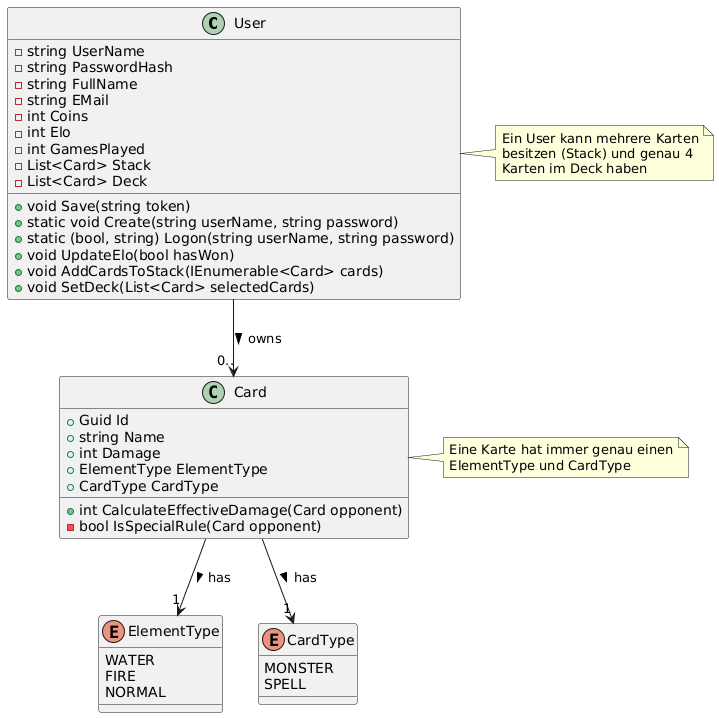
\includegraphics[width=\textwidth]{UML.png}
    \label{fig:uml}
\end{center}


\end{document}